\hypertarget{czasteczka_8cpp}{\section{Dokumentacja pliku czasteczka.\-cpp}
\label{czasteczka_8cpp}\index{czasteczka.\-cpp@{czasteczka.\-cpp}}
}


Zawiera definicje metod klasy \hyperlink{class_czasteczka}{Czasteczka}.  


{\ttfamily \#include \char`\"{}czasteczka.\-hh\char`\"{}}\\*
Wykres zależności załączania dla czasteczka.\-cpp\-:\nopagebreak
\begin{figure}[H]
\begin{center}
\leavevmode
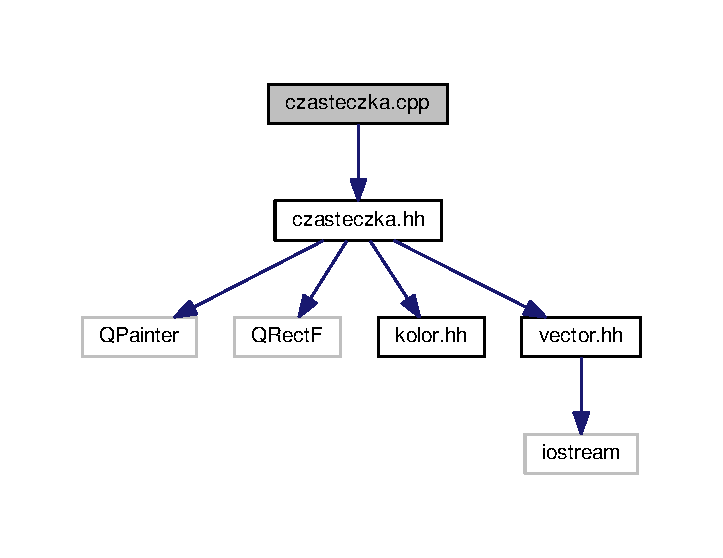
\includegraphics[width=347pt]{czasteczka_8cpp__incl}
\end{center}
\end{figure}


\subsection{Opis szczegółowy}
W pliku znajduja sie\-:
\begin{DoxyItemize}
\item metoda rysujaca czasteczkę. 
\end{DoxyItemize}

Definicja w pliku \hyperlink{czasteczka_8cpp_source}{czasteczka.\-cpp}.

